\documentclass[]{article}
\usepackage{lmodern}
\usepackage{amssymb,amsmath}
\usepackage{ifxetex,ifluatex}
\usepackage{fixltx2e} % provides \textsubscript
\ifnum 0\ifxetex 1\fi\ifluatex 1\fi=0 % if pdftex
  \usepackage[T1]{fontenc}
  \usepackage[utf8]{inputenc}
\else % if luatex or xelatex
  \ifxetex
    \usepackage{mathspec}
  \else
    \usepackage{fontspec}
  \fi
  \defaultfontfeatures{Ligatures=TeX,Scale=MatchLowercase}
\fi
% use upquote if available, for straight quotes in verbatim environments
\IfFileExists{upquote.sty}{\usepackage{upquote}}{}
% use microtype if available
\IfFileExists{microtype.sty}{%
\usepackage{microtype}
\UseMicrotypeSet[protrusion]{basicmath} % disable protrusion for tt fonts
}{}
\usepackage[margin=1in]{geometry}
\usepackage{hyperref}
\hypersetup{unicode=true,
            pdftitle={Class6 R functions},
            pdfauthor={Hongji Jiang},
            pdfborder={0 0 0},
            breaklinks=true}
\urlstyle{same}  % don't use monospace font for urls
\usepackage{color}
\usepackage{fancyvrb}
\newcommand{\VerbBar}{|}
\newcommand{\VERB}{\Verb[commandchars=\\\{\}]}
\DefineVerbatimEnvironment{Highlighting}{Verbatim}{commandchars=\\\{\}}
% Add ',fontsize=\small' for more characters per line
\usepackage{framed}
\definecolor{shadecolor}{RGB}{248,248,248}
\newenvironment{Shaded}{\begin{snugshade}}{\end{snugshade}}
\newcommand{\KeywordTok}[1]{\textcolor[rgb]{0.13,0.29,0.53}{\textbf{#1}}}
\newcommand{\DataTypeTok}[1]{\textcolor[rgb]{0.13,0.29,0.53}{#1}}
\newcommand{\DecValTok}[1]{\textcolor[rgb]{0.00,0.00,0.81}{#1}}
\newcommand{\BaseNTok}[1]{\textcolor[rgb]{0.00,0.00,0.81}{#1}}
\newcommand{\FloatTok}[1]{\textcolor[rgb]{0.00,0.00,0.81}{#1}}
\newcommand{\ConstantTok}[1]{\textcolor[rgb]{0.00,0.00,0.00}{#1}}
\newcommand{\CharTok}[1]{\textcolor[rgb]{0.31,0.60,0.02}{#1}}
\newcommand{\SpecialCharTok}[1]{\textcolor[rgb]{0.00,0.00,0.00}{#1}}
\newcommand{\StringTok}[1]{\textcolor[rgb]{0.31,0.60,0.02}{#1}}
\newcommand{\VerbatimStringTok}[1]{\textcolor[rgb]{0.31,0.60,0.02}{#1}}
\newcommand{\SpecialStringTok}[1]{\textcolor[rgb]{0.31,0.60,0.02}{#1}}
\newcommand{\ImportTok}[1]{#1}
\newcommand{\CommentTok}[1]{\textcolor[rgb]{0.56,0.35,0.01}{\textit{#1}}}
\newcommand{\DocumentationTok}[1]{\textcolor[rgb]{0.56,0.35,0.01}{\textbf{\textit{#1}}}}
\newcommand{\AnnotationTok}[1]{\textcolor[rgb]{0.56,0.35,0.01}{\textbf{\textit{#1}}}}
\newcommand{\CommentVarTok}[1]{\textcolor[rgb]{0.56,0.35,0.01}{\textbf{\textit{#1}}}}
\newcommand{\OtherTok}[1]{\textcolor[rgb]{0.56,0.35,0.01}{#1}}
\newcommand{\FunctionTok}[1]{\textcolor[rgb]{0.00,0.00,0.00}{#1}}
\newcommand{\VariableTok}[1]{\textcolor[rgb]{0.00,0.00,0.00}{#1}}
\newcommand{\ControlFlowTok}[1]{\textcolor[rgb]{0.13,0.29,0.53}{\textbf{#1}}}
\newcommand{\OperatorTok}[1]{\textcolor[rgb]{0.81,0.36,0.00}{\textbf{#1}}}
\newcommand{\BuiltInTok}[1]{#1}
\newcommand{\ExtensionTok}[1]{#1}
\newcommand{\PreprocessorTok}[1]{\textcolor[rgb]{0.56,0.35,0.01}{\textit{#1}}}
\newcommand{\AttributeTok}[1]{\textcolor[rgb]{0.77,0.63,0.00}{#1}}
\newcommand{\RegionMarkerTok}[1]{#1}
\newcommand{\InformationTok}[1]{\textcolor[rgb]{0.56,0.35,0.01}{\textbf{\textit{#1}}}}
\newcommand{\WarningTok}[1]{\textcolor[rgb]{0.56,0.35,0.01}{\textbf{\textit{#1}}}}
\newcommand{\AlertTok}[1]{\textcolor[rgb]{0.94,0.16,0.16}{#1}}
\newcommand{\ErrorTok}[1]{\textcolor[rgb]{0.64,0.00,0.00}{\textbf{#1}}}
\newcommand{\NormalTok}[1]{#1}
\usepackage{graphicx,grffile}
\makeatletter
\def\maxwidth{\ifdim\Gin@nat@width>\linewidth\linewidth\else\Gin@nat@width\fi}
\def\maxheight{\ifdim\Gin@nat@height>\textheight\textheight\else\Gin@nat@height\fi}
\makeatother
% Scale images if necessary, so that they will not overflow the page
% margins by default, and it is still possible to overwrite the defaults
% using explicit options in \includegraphics[width, height, ...]{}
\setkeys{Gin}{width=\maxwidth,height=\maxheight,keepaspectratio}
\IfFileExists{parskip.sty}{%
\usepackage{parskip}
}{% else
\setlength{\parindent}{0pt}
\setlength{\parskip}{6pt plus 2pt minus 1pt}
}
\setlength{\emergencystretch}{3em}  % prevent overfull lines
\providecommand{\tightlist}{%
  \setlength{\itemsep}{0pt}\setlength{\parskip}{0pt}}
\setcounter{secnumdepth}{0}
% Redefines (sub)paragraphs to behave more like sections
\ifx\paragraph\undefined\else
\let\oldparagraph\paragraph
\renewcommand{\paragraph}[1]{\oldparagraph{#1}\mbox{}}
\fi
\ifx\subparagraph\undefined\else
\let\oldsubparagraph\subparagraph
\renewcommand{\subparagraph}[1]{\oldsubparagraph{#1}\mbox{}}
\fi

%%% Use protect on footnotes to avoid problems with footnotes in titles
\let\rmarkdownfootnote\footnote%
\def\footnote{\protect\rmarkdownfootnote}

%%% Change title format to be more compact
\usepackage{titling}

% Create subtitle command for use in maketitle
\providecommand{\subtitle}[1]{
  \posttitle{
    \begin{center}\large#1\end{center}
    }
}

\setlength{\droptitle}{-2em}

  \title{Class6 R functions}
    \pretitle{\vspace{\droptitle}\centering\huge}
  \posttitle{\par}
    \author{Hongji Jiang}
    \preauthor{\centering\large\emph}
  \postauthor{\par}
      \predate{\centering\large\emph}
  \postdate{\par}
    \date{10/17/2019}


\begin{document}
\maketitle

\section{\texorpdfstring{This is my work from class6
\textbf{BIMM143}.}{This is my work from class6 BIMM143.}}\label{this-is-my-work-from-class6-bimm143.}

\begin{Shaded}
\begin{Highlighting}[]
\CommentTok{#this is to demo a code chunk}
\KeywordTok{plot}\NormalTok{(}\DecValTok{1}\OperatorTok{:}\DecValTok{10}\NormalTok{)}
\end{Highlighting}
\end{Shaded}

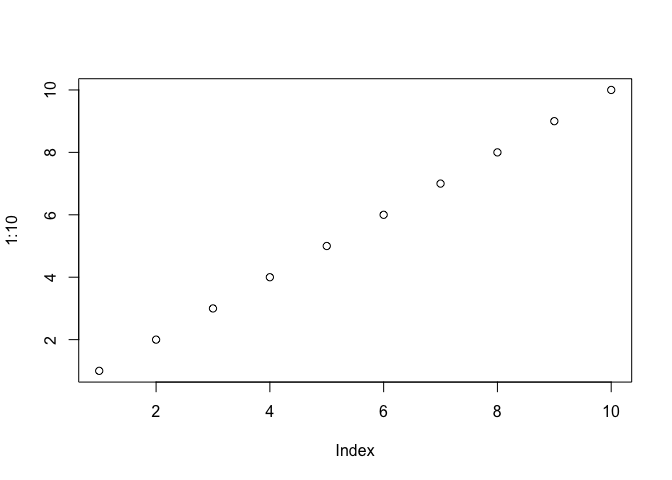
\includegraphics{class6_files/figure-latex/unnamed-chunk-1-1.pdf}

\subsection{Practice Reading
Files(again\ldots{})}\label{practice-reading-filesagain}

\begin{Shaded}
\begin{Highlighting}[]
\KeywordTok{read.table}\NormalTok{(}\StringTok{"test1.txt"}\NormalTok{,}\DataTypeTok{sep =} \StringTok{","}\NormalTok{, }\DataTypeTok{header =} \OtherTok{TRUE}\NormalTok{)}
\end{Highlighting}
\end{Shaded}

\begin{verbatim}
##   Col1 Col2 Col3
## 1    1    2    3
## 2    4    5    6
## 3    7    8    9
## 4    a    b    c
\end{verbatim}

\begin{Shaded}
\begin{Highlighting}[]
\KeywordTok{read.table}\NormalTok{(}\StringTok{"test2.txt"}\NormalTok{,}\DataTypeTok{sep =} \StringTok{"$"}\NormalTok{, }\DataTypeTok{header =} \OtherTok{TRUE}\NormalTok{)}
\end{Highlighting}
\end{Shaded}

\begin{verbatim}
##   Col1 Col2 Col3
## 1    1    2    3
## 2    4    5    6
## 3    7    8    9
## 4    a    b    c
\end{verbatim}

\begin{Shaded}
\begin{Highlighting}[]
\KeywordTok{read.table}\NormalTok{(}\StringTok{"test3.txt"}\NormalTok{)}
\end{Highlighting}
\end{Shaded}

\begin{verbatim}
##   V1 V2 V3
## 1  1  6  a
## 2  2  7  b
## 3  3  8  c
## 4  4  9  d
## 5  5 10  e
\end{verbatim}

\begin{Shaded}
\begin{Highlighting}[]
\NormalTok{add <-}\StringTok{ }\ControlFlowTok{function}\NormalTok{(x, }\DataTypeTok{y=}\DecValTok{1}\NormalTok{) \{}
\CommentTok{# Sum the input x and y }
\NormalTok{  x}\OperatorTok{+}\NormalTok{y}
\NormalTok{\}}
\end{Highlighting}
\end{Shaded}

\begin{Shaded}
\begin{Highlighting}[]
\KeywordTok{add}\NormalTok{(}\DecValTok{1}\NormalTok{)}
\end{Highlighting}
\end{Shaded}

\begin{verbatim}
## [1] 2
\end{verbatim}

\begin{Shaded}
\begin{Highlighting}[]
\KeywordTok{add}\NormalTok{(}\DecValTok{5}\NormalTok{,}\DecValTok{5}\NormalTok{)}
\end{Highlighting}
\end{Shaded}

\begin{verbatim}
## [1] 10
\end{verbatim}

\begin{Shaded}
\begin{Highlighting}[]
\NormalTok{rescale <-}\StringTok{ }\ControlFlowTok{function}\NormalTok{(x) \{}
\NormalTok{   rng <-}\KeywordTok{range}\NormalTok{(x)}
\NormalTok{   (x }\OperatorTok{-}\StringTok{ }\NormalTok{rng[}\DecValTok{1}\NormalTok{]) }\OperatorTok{/}\StringTok{ }\NormalTok{(rng[}\DecValTok{2}\NormalTok{] }\OperatorTok{-}\StringTok{ }\NormalTok{rng[}\DecValTok{1}\NormalTok{])}
\NormalTok{\}}
\end{Highlighting}
\end{Shaded}

\begin{Shaded}
\begin{Highlighting}[]
\KeywordTok{rescale}\NormalTok{(}\DecValTok{1}\OperatorTok{:}\DecValTok{10}\NormalTok{)}
\end{Highlighting}
\end{Shaded}

\begin{verbatim}
##  [1] 0.0000000 0.1111111 0.2222222 0.3333333 0.4444444 0.5555556 0.6666667
##  [8] 0.7777778 0.8888889 1.0000000
\end{verbatim}

Test some

\begin{Shaded}
\begin{Highlighting}[]
\NormalTok{x<-}\KeywordTok{c}\NormalTok{(}\DecValTok{1}\NormalTok{,}\DecValTok{2}\NormalTok{,}\OtherTok{NA}\NormalTok{,}\DecValTok{3}\NormalTok{,}\DecValTok{10}\NormalTok{)}
\KeywordTok{rescale}\NormalTok{(}\KeywordTok{c}\NormalTok{(}\DecValTok{1}\NormalTok{,}\DecValTok{2}\NormalTok{,}\OtherTok{NA}\NormalTok{,}\DecValTok{3}\NormalTok{,}\DecValTok{10}\NormalTok{))}
\end{Highlighting}
\end{Shaded}

\begin{verbatim}
## [1] NA NA NA NA NA
\end{verbatim}

\begin{Shaded}
\begin{Highlighting}[]
\NormalTok{rng =}\StringTok{ }\KeywordTok{range}\NormalTok{(x,}\DataTypeTok{na.rm =} \OtherTok{TRUE}\NormalTok{)}
\NormalTok{rng}
\end{Highlighting}
\end{Shaded}

\begin{verbatim}
## [1]  1 10
\end{verbatim}

\begin{Shaded}
\begin{Highlighting}[]
\NormalTok{rescale2 <-}\StringTok{ }\ControlFlowTok{function}\NormalTok{(x) \{}
\NormalTok{   rng <-}\KeywordTok{range}\NormalTok{(x,}\DataTypeTok{na.rm =} \OtherTok{TRUE}\NormalTok{)}
\NormalTok{   (x }\OperatorTok{-}\StringTok{ }\NormalTok{rng[}\DecValTok{1}\NormalTok{]) }\OperatorTok{/}\StringTok{ }\NormalTok{(rng[}\DecValTok{2}\NormalTok{] }\OperatorTok{-}\StringTok{ }\NormalTok{rng[}\DecValTok{1}\NormalTok{])}
\NormalTok{\}}
\end{Highlighting}
\end{Shaded}

\begin{Shaded}
\begin{Highlighting}[]
\KeywordTok{rescale2}\NormalTok{(x)}
\end{Highlighting}
\end{Shaded}

\begin{verbatim}
## [1] 0.0000000 0.1111111        NA 0.2222222 1.0000000
\end{verbatim}

\begin{Shaded}
\begin{Highlighting}[]
\NormalTok{ rescale3 <-}\StringTok{ }\ControlFlowTok{function}\NormalTok{(x, }\DataTypeTok{na.rm=}\OtherTok{TRUE}\NormalTok{, }\DataTypeTok{plot=}\OtherTok{FALSE}\NormalTok{) \{}
\NormalTok{    rng <-}\KeywordTok{range}\NormalTok{(x, }\DataTypeTok{na.rm=}\NormalTok{na.rm)}
    \KeywordTok{print}\NormalTok{(}\StringTok{"Hello"}\NormalTok{)}
\NormalTok{   answer <-}\StringTok{ }\NormalTok{(x }\OperatorTok{-}\StringTok{ }\NormalTok{rng[}\DecValTok{1}\NormalTok{]) }\OperatorTok{/}\StringTok{ }\NormalTok{(rng[}\DecValTok{2}\NormalTok{] }\OperatorTok{-}\StringTok{ }\NormalTok{rng[}\DecValTok{1}\NormalTok{])}
   \KeywordTok{print}\NormalTok{(}\StringTok{"is it me you are looking for?"}\NormalTok{)}
   \ControlFlowTok{if}\NormalTok{(plot) \{}
      \KeywordTok{plot}\NormalTok{(answer, }\DataTypeTok{typ=}\StringTok{"b"}\NormalTok{, }\DataTypeTok{lwd=}\DecValTok{4}\NormalTok{)}
\NormalTok{   \}}
   \KeywordTok{print}\NormalTok{(}\StringTok{"I can see it in ..."}\NormalTok{)}
   \KeywordTok{return}\NormalTok{(answer)}
\NormalTok{\}}
\end{Highlighting}
\end{Shaded}

\begin{Shaded}
\begin{Highlighting}[]
\KeywordTok{rescale3}\NormalTok{(}\DecValTok{1}\OperatorTok{:}\DecValTok{10}\NormalTok{,}\DataTypeTok{plot=}\OtherTok{TRUE}\NormalTok{)}
\end{Highlighting}
\end{Shaded}

\begin{verbatim}
## [1] "Hello"
## [1] "is it me you are looking for?"
\end{verbatim}

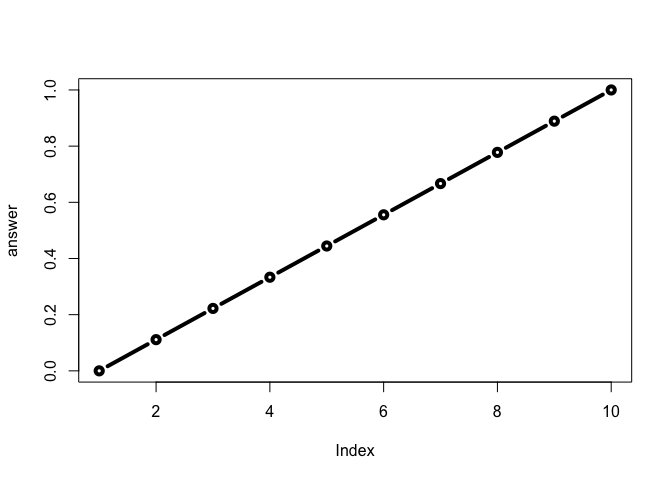
\includegraphics{class6_files/figure-latex/unnamed-chunk-11-1.pdf}

\begin{verbatim}
## [1] "I can see it in ..."
\end{verbatim}

\begin{verbatim}
##  [1] 0.0000000 0.1111111 0.2222222 0.3333333 0.4444444 0.5555556 0.6666667
##  [8] 0.7777778 0.8888889 1.0000000
\end{verbatim}

\section{section2}\label{section2}

Install the \textbf{bio3d} pakage for sequence and structure analysis

\begin{Shaded}
\begin{Highlighting}[]
\KeywordTok{library}\NormalTok{(bio3d)}
\NormalTok{s1 <-}\StringTok{ }\KeywordTok{read.pdb}\NormalTok{(}\StringTok{"4AKE"}\NormalTok{)  }\CommentTok{# kinase with drug}
\end{Highlighting}
\end{Shaded}

\begin{verbatim}
##   Note: Accessing on-line PDB file
\end{verbatim}

\begin{Shaded}
\begin{Highlighting}[]
\NormalTok{s2 <-}\StringTok{ }\KeywordTok{read.pdb}\NormalTok{(}\StringTok{"1AKE"}\NormalTok{)  }\CommentTok{# kinase no drug}
\end{Highlighting}
\end{Shaded}

\begin{verbatim}
##   Note: Accessing on-line PDB file
##    PDB has ALT records, taking A only, rm.alt=TRUE
\end{verbatim}

\begin{Shaded}
\begin{Highlighting}[]
\NormalTok{s3 <-}\StringTok{ }\KeywordTok{read.pdb}\NormalTok{(}\StringTok{"1E4Y"}\NormalTok{)  }\CommentTok{# kinase with drug}
\end{Highlighting}
\end{Shaded}

\begin{verbatim}
##   Note: Accessing on-line PDB file
\end{verbatim}

\begin{Shaded}
\begin{Highlighting}[]
\NormalTok{s1.chainA <-}\StringTok{ }\KeywordTok{trim.pdb}\NormalTok{(s1, }\DataTypeTok{chain=}\StringTok{"A"}\NormalTok{, }\DataTypeTok{elety=}\StringTok{"CA"}\NormalTok{)}
\NormalTok{s2.chainA <-}\StringTok{ }\KeywordTok{trim.pdb}\NormalTok{(s2, }\DataTypeTok{chain=}\StringTok{"A"}\NormalTok{, }\DataTypeTok{elety=}\StringTok{"CA"}\NormalTok{)}
\NormalTok{s3.chainA <-}\StringTok{ }\KeywordTok{trim.pdb}\NormalTok{(s3, }\DataTypeTok{chain=}\StringTok{"A"}\NormalTok{, }\DataTypeTok{elety=}\StringTok{"CA"}\NormalTok{)}
\NormalTok{s1.b <-}\StringTok{ }\NormalTok{s1.chainA}\OperatorTok{$}\NormalTok{atom}\OperatorTok{$}\NormalTok{b}
\NormalTok{s2.b <-}\StringTok{ }\NormalTok{s2.chainA}\OperatorTok{$}\NormalTok{atom}\OperatorTok{$}\NormalTok{b}
\NormalTok{s3.b <-}\StringTok{ }\NormalTok{s3.chainA}\OperatorTok{$}\NormalTok{atom}\OperatorTok{$}\NormalTok{b}
\KeywordTok{plotb3}\NormalTok{(s1.b, }\DataTypeTok{sse=}\NormalTok{s1.chainA, }\DataTypeTok{typ=}\StringTok{"l"}\NormalTok{, }\DataTypeTok{ylab=}\StringTok{"Bfactor"}\NormalTok{)}
\end{Highlighting}
\end{Shaded}

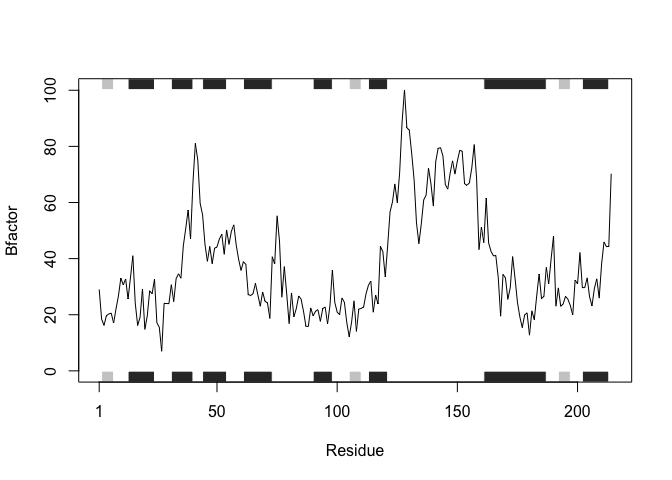
\includegraphics{class6_files/figure-latex/unnamed-chunk-12-1.pdf}

\begin{Shaded}
\begin{Highlighting}[]
\KeywordTok{plotb3}\NormalTok{(s2.b, }\DataTypeTok{sse=}\NormalTok{s2.chainA, }\DataTypeTok{typ=}\StringTok{"l"}\NormalTok{, }\DataTypeTok{ylab=}\StringTok{"Bfactor"}\NormalTok{)}
\end{Highlighting}
\end{Shaded}

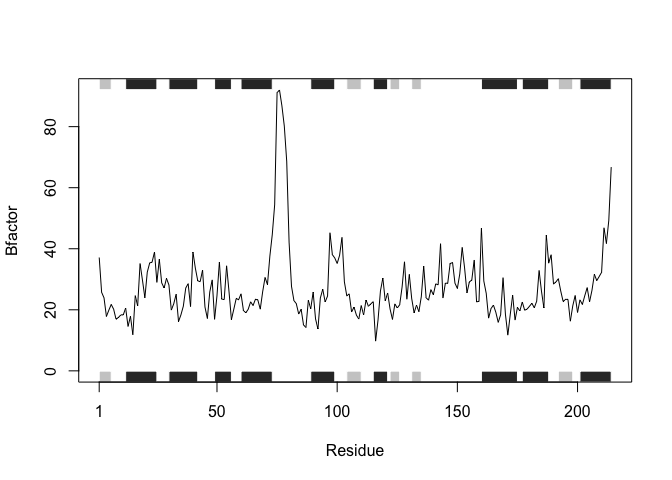
\includegraphics{class6_files/figure-latex/unnamed-chunk-12-2.pdf}

\begin{Shaded}
\begin{Highlighting}[]
\KeywordTok{plotb3}\NormalTok{(s3.b, }\DataTypeTok{sse=}\NormalTok{s3.chainA, }\DataTypeTok{typ=}\StringTok{"l"}\NormalTok{, }\DataTypeTok{ylab=}\StringTok{"Bfactor"}\NormalTok{)}
\end{Highlighting}
\end{Shaded}

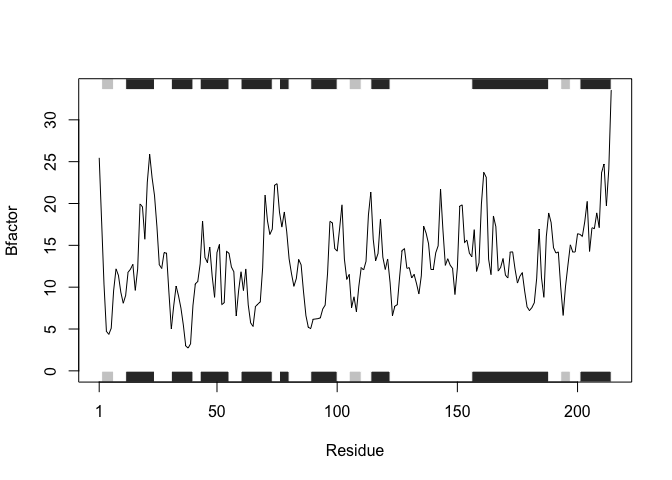
\includegraphics{class6_files/figure-latex/unnamed-chunk-12-3.pdf}

\begin{Shaded}
\begin{Highlighting}[]
\NormalTok{hc <-}\StringTok{ }\KeywordTok{hclust}\NormalTok{( }\KeywordTok{dist}\NormalTok{( }\KeywordTok{rbind}\NormalTok{(s1.b, s2.b, s3.b) ) )}
\KeywordTok{plot}\NormalTok{(hc)}
\end{Highlighting}
\end{Shaded}

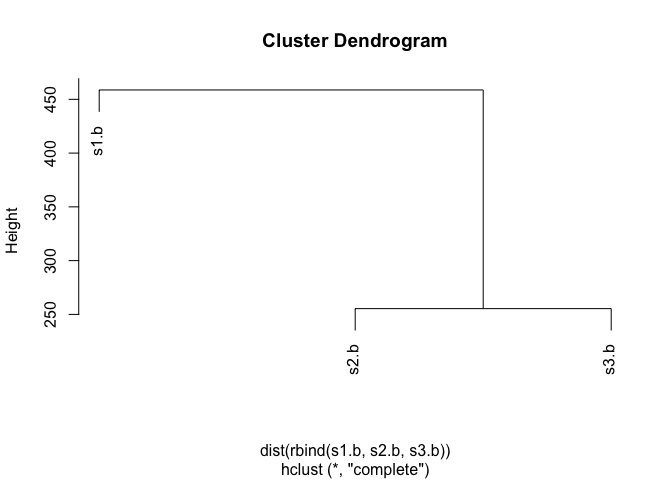
\includegraphics{class6_files/figure-latex/unnamed-chunk-13-1.pdf}

\begin{Shaded}
\begin{Highlighting}[]
\CommentTok{# function describtion }
\CommentTok{# this function takes in one argument x that is the name }
\CommentTok{# of the pdb file }
\CommentTok{# Output: it plots a plot with residue on x-label and }
\CommentTok{# Bfactor on the y-label}
\NormalTok{plotp <-}\StringTok{ }\ControlFlowTok{function}\NormalTok{(x)}
\NormalTok{\{}
  \CommentTok{# read.pdb reads a protein data bank coordinate file}
  \CommentTok{# argument x is the name of the PDB file to read }
\NormalTok{  s =}\StringTok{ }\KeywordTok{read.pdb}\NormalTok{(x)}
  \CommentTok{# trim.pdb produces a smaller pdb object}
  \CommentTok{# it contains a subset of atoms }
  \CommentTok{# argument elety: a character vector of atom names.}
  \CommentTok{# argument chain a character vecter of chain identifiers}
\NormalTok{  s.chainA <-}\StringTok{ }\KeywordTok{trim.pdb}\NormalTok{(s, }\DataTypeTok{chain=}\StringTok{"A"}\NormalTok{, }\DataTypeTok{elety=}\StringTok{"CA"}\NormalTok{)}
\NormalTok{  s.b <-}\StringTok{ }\NormalTok{s.chainA}\OperatorTok{$}\NormalTok{atom}\OperatorTok{$}\NormalTok{b}
  \CommentTok{# plotb3: Draw a standard scatter plot}
  \CommentTok{# with optional secondary structure in the marginal regions.}
  \KeywordTok{plotb3}\NormalTok{(s.b, }\DataTypeTok{sse=}\NormalTok{s.chainA, }\DataTypeTok{typ=}\StringTok{"l"}\NormalTok{, }\DataTypeTok{ylab=}\StringTok{"Bfactor"}\NormalTok{)}
\NormalTok{\}}
\CommentTok{# Here I use the three examples above }
\CommentTok{# to test my function}
\KeywordTok{plotp}\NormalTok{(}\StringTok{"4AKE"}\NormalTok{)}
\end{Highlighting}
\end{Shaded}

\begin{verbatim}
##   Note: Accessing on-line PDB file
\end{verbatim}

\begin{verbatim}
## Warning in get.pdb(file, path = tempdir(), verbose = FALSE): /var/folders/
## d1/r9lcn8313z5_hg24vb00hp8w0000gn/T//RtmpJo9ddF/4AKE.pdb exists. Skipping
## download
\end{verbatim}

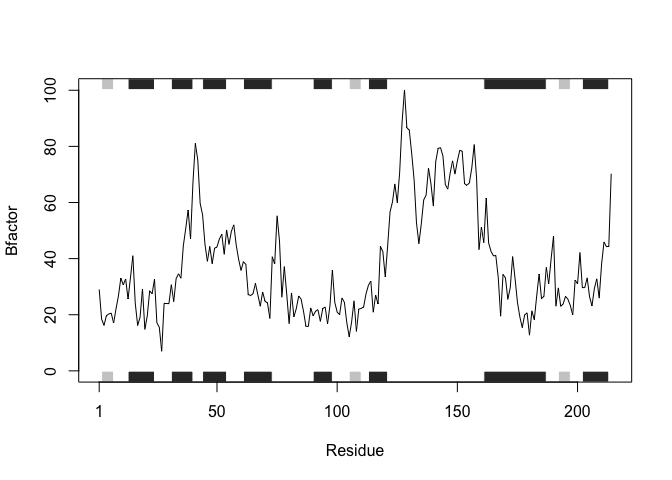
\includegraphics{class6_files/figure-latex/unnamed-chunk-14-1.pdf}

\begin{Shaded}
\begin{Highlighting}[]
\KeywordTok{plotp}\NormalTok{(}\StringTok{"1AKE"}\NormalTok{)}
\end{Highlighting}
\end{Shaded}

\begin{verbatim}
##   Note: Accessing on-line PDB file
\end{verbatim}

\begin{verbatim}
## Warning in get.pdb(file, path = tempdir(), verbose = FALSE): /var/folders/
## d1/r9lcn8313z5_hg24vb00hp8w0000gn/T//RtmpJo9ddF/1AKE.pdb exists. Skipping
## download
\end{verbatim}

\begin{verbatim}
##    PDB has ALT records, taking A only, rm.alt=TRUE
\end{verbatim}

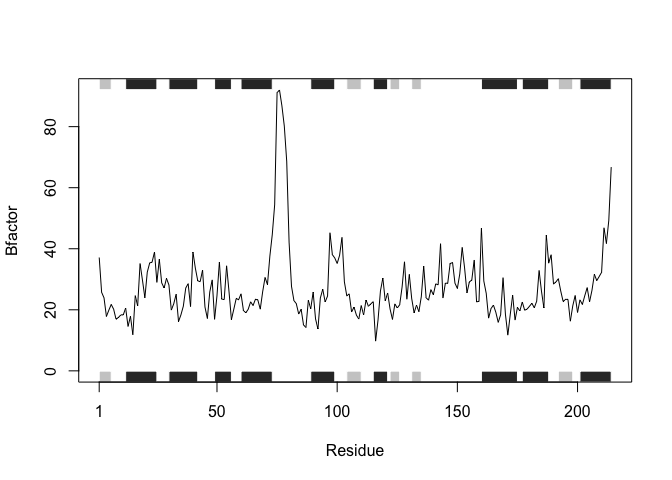
\includegraphics{class6_files/figure-latex/unnamed-chunk-14-2.pdf}

\begin{Shaded}
\begin{Highlighting}[]
\KeywordTok{plotp}\NormalTok{(}\StringTok{"1E4Y"}\NormalTok{)}
\end{Highlighting}
\end{Shaded}

\begin{verbatim}
##   Note: Accessing on-line PDB file
\end{verbatim}

\begin{verbatim}
## Warning in get.pdb(file, path = tempdir(), verbose = FALSE): /var/folders/
## d1/r9lcn8313z5_hg24vb00hp8w0000gn/T//RtmpJo9ddF/1E4Y.pdb exists. Skipping
## download
\end{verbatim}

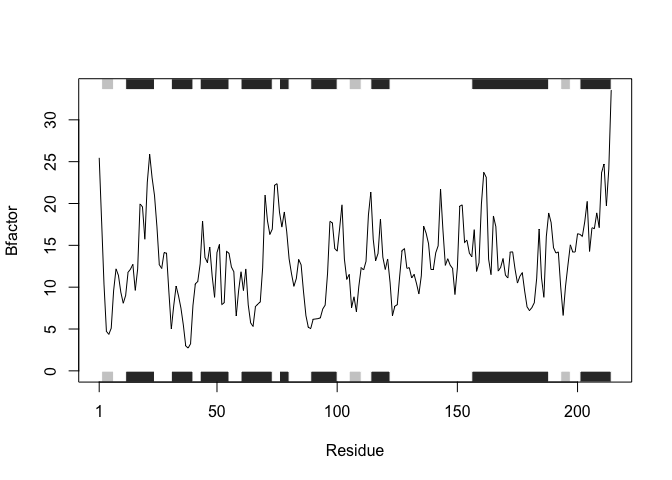
\includegraphics{class6_files/figure-latex/unnamed-chunk-14-3.pdf}


\end{document}
